\section{Motivation and Problem Formulation}\label{sec:motivation}

In flow-based microfluidic biochips, flow channels and control channels are
etched upon a substrate from PDMS through a process that includes molding and
assembling \cite{C2LC40258K}. 
%Air pressure is conducted through control channesl to the membrane layer at
%the intersections between flow and control channels to activate valves. 
In this multiple-step process, defects may appear in the manufactured chips.
For example, flow channels may be broken during the molding process; flow
and control layers may also be aligned improperly so that the pressure conducted
through control channels cannot reach the corresponding valves, leading
to valves that cannot be closed.  Figure~\ref{fig:defects} shows cases with
broken flow and control channels \cite{HuYHC14}, two typical defects after
manufacturing, leading to defects such as flow channels that are blocked and
valves that cannot be closed.

\begin{figure}
\figurefontsize
\centering
\input{Fig/defects.pdf_tex}
\caption{Manufacturing defects in continuous-flow biochips \cite{HuYHC14}. (a)
Broken flow channel. (b) Broken control channel.}
\label{fig:defects}
\end{figure}

To identify biochips with defects after manufacturing, a given set of test
vectors needs to be applied, each of which is a combination of valve states.
In the test procedure, air pressure sources are connected to some ports of the
chip.  A test vector is then applied to open and close the valves to create
flow paths inside the chip to test the defects where channels are blocked or
valves cannot be opened.  Pressure meters are attached to other ports of the
chip and the measured pressure results are compared with a predetermined set
of measurements. If discrepancy exists, the chip is then reported to have
defects. Reciprocally, to test the defects that valves cannot be closed, some
valves are closed to separate the pressure sources and meters. If pressure can
still be measured, a defect is thus detected.  In this test procedure, usually
air pressure instead of fluid is used to keep the chip from being contaminated
before they are sold on the market.

%In the test procedure, the measured pressure at test ports are evaluated as
%binary results. The intermediate levels of pressure values are not considered
%to reduce the complexity and uncertainty. Consequently, the test procedure of
%such biochips is very similar to the test procedure of integrated circuits.
%Accordingly, these test methods proposed in 
%\cite{HuYHC14,HuHC14} convert this test problem into a digital circuit and
%applied ATPG methods to generate test vectors directly. 
%On the contrary, the
%method in \cite{Liudate17} examines the relation between the test vectors and
%the pressure measurements directy and construct test vectors accordingly.
%These methods, however, do not consider cost reduction in the overall test
%platform.

%The test procedure usually consists three steps: (1) External ports on the chip are
%connected to pressure sources and meters; (2) Test vectors are applied and
%the open/closed states of valves are inside the chip are changed accordingly;
%(3) Air pressrue is pushed into the chip. If there are flow paths from a
%pressure source to a pressure mether on which all valves are open, the meter
%is supposed to detect the pressure; otherwise, if there is no open path from a
%pressure source to the meter, it thus returns no pressure reading. This result
%is compared with a predetermined value for this test vector, and a mismatch in
%any of the meter outputs indicates a defect in chip.

The test procedure can be explained using
\figname~\ref{fig:multiPortSingPort}(a), where the biochip has three ports and
six valves.  
%The rectangular blocks in this chip represent valves. 
%and the valves with filled color are closed. 
%where test vectors are applied to test a biochip with three ports. 
Since a valve allows pressure propagation in either direction, the ports of a
biochip are equivalent in the test procedure, so that each of them can be
connected to either a pressure source or a pressure meter.  In 
\figname~\ref{fig:multiPortSingPort}(a), 
one of the ports of the biochip is connected to a pressure source 
and the other two are connected to pressure meters. 

To detect the defects in which valves cannot be opened,
two test vectors, path P1 and path P2, are generated for the biochip in  
\figname~\ref{fig:multiPortSingPort}(a). When such a test vector is applied, all
the other valves that are not on the path are closed. If a valve on the path
cannot be opened due to manufacturing defects, the pressure meters cannot
measure any pressure, because no other path from the pressure source to the
meter exists. Similar to test paths, test vectors also contain cuts to verify
whether valves can be opened correctly. For example, if the valves in 
one of the four cuts
C1--C4 in \figname~\ref{fig:multiPortSingPort}(a) are closed, the chip is
separated into two parts and the pressure from the source should not reach any
pressure meter.  If a pressure meter still reads a valid pressure value, a
defect is then detected. For convenience, we call a valve that cannot be opened
or a channel that is blocked a stuck-at-0 defect, and a valve that cannot be
closed a stuck-at-1 defect. Besides these defects, there are also leakage
defects between flow channels and control channels, which also affect the
function of a chip and can be tested similarly \cite{HuYHC14}. In this paper,
we will use only stuck-at-0 and stuck-at-1 defects to demonstrate the proposed
design-for-testability method.

\begin{figure}
\figurefontsize
\centering
%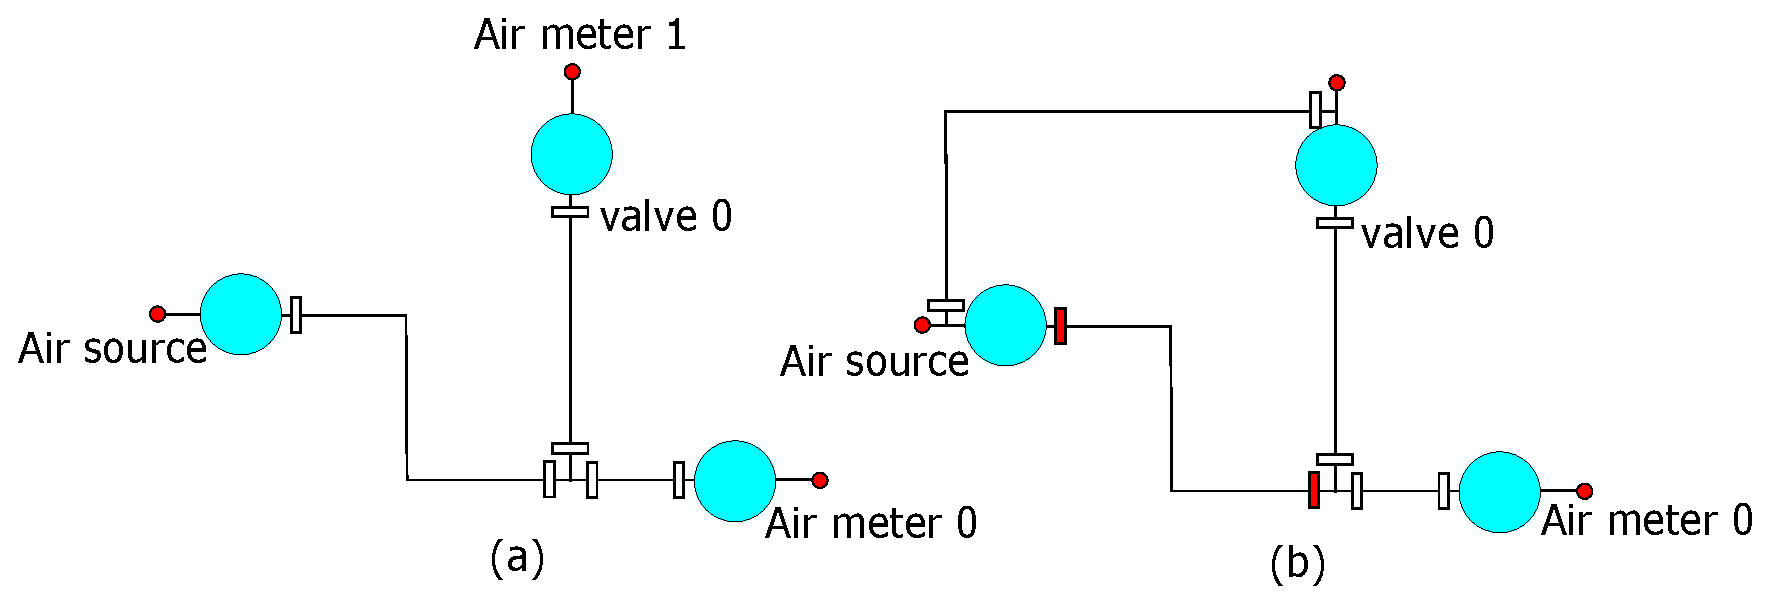
\includegraphics[width=3.50in,height=1.2in]{Fig/multiport_single_port1.eps}
\input{Fig/multiport_single_port.pdf_tex}
\caption{Test vectors and design-for-testability.  
  (a) Test paths and cuts to detect stuck-at-0 and stuck-at-1
  defects. 
  (b) Single-source single-meter test.}
\label{fig:multiPortSingPort}
\end{figure}

In \figname~\ref{fig:multiPortSingPort}(a), one pressure source and two
pressure meters are required. These mechanical devices are cumbersome and the
installation as well as their connection to the biochip under test makes the
test procedure error-prone. Therefore, it is beneficial to reduce the number of
such devices to the minimum in the test platform.  To achieve this reduction,
the architecture of the biochip in \figname~\ref{fig:multiPortSingPort}(a) can
be modified to add more channels and valves, so that only one pressure source and
one meter are required, as shown in \figname~\ref{fig:multiPortSingPort}(b).
With this reduction, test paths P1-P2 and cuts C1-C6 can still be generated
successfully to detect manufacturing defects. Obviously this modification
introduces more channels and valves into the chip. However, the cost of the
chip does not increase noticeably, because biochips are manufactured 
using masks as for IC manufacturing, and a large number of valves can already
be built in a chip cost-effectively \cite{JEMP08}.
%where most of the cost comes from the
%generation of the masks, if the  
%no matter how many devices and channels are on
%the mask, provided that the area occupied by the chips does not change.
The increased number of test vectors is also affordable, since
test time is still not the first concern in  
state-of-the-art biochip design \cite{HuYHC14}.
%the test time is still not a concern currently. 
%still allows for more than 10 minutes for each chip to be tested 
%\cite{HuYHC14}.

The valves introduced in the modified chip architecture still need to be
controlled by control ports connected to them, as illustrated in
\figname~\ref{fig:valve_mixer_chip}. In the case where additional independent
control ports can be provided,
%in application environment, 
the two valves and channels in \figname~\ref{fig:multiPortSingPort}(b)
provide new resources for the execution of applications. Therefore, the
performance of the biochip can be improved accordingly. If, on the other hand,
the control logic is not capable of providing additional independent control
ports, the new valves introduced to increase testability should share a control
port together with another existing valve in the original biochip. This
sharing still needs to allow a valid set of test vectors to be generated to
test all the stuck-at-0 and stuck-at-1 defects.
%and the execution efficientcy of application should still be maintained.

%In addition, 
When an application is executed by the modified biochip, 
%the modified chip architecture and the shared valves
it should provide similar performance compared with the version before
modification.  The sharing of control logic between a newly added valve and an
existing valve, however, limits the flexibility in transporting fluid results
between devices, because contamination may occur due to the valves that
are forced to open together with another valve. Similarly, the forced close state of
shared valve increases the chance of blocking in fluid transportation, thus
also leading to a low execution efficiency of the application.

With the discussion above, we can then formulate the design-for-testability
problem as follows.

\noindent\textit{Given}: A biochip architecture with the application to be
executed.

\noindent\textit{Output}: An augmented biochip architecture for testability; a set of test
vectors considering valve sharing; a schedule of the application on the
augmented biochip architecture.

\noindent\textit{Objectives}: The augmented architecture requires only a
single pressure source and a single pressure meter for testing 
manufacturing defects; the execution efficiency of the application should be
maintained at the same level.

